\documentclass[main]{subfiles}

\begin{document}

\chapter{GPS}
\label{chap-gps}

\section{Objetivos}

En este capítulo se analiza la performance del GPS Canmore GT-730F. Se intenta reconstruir un polígono, y se analiza el error al estimar la posición de un punto fijo.

\section{Materiales}

\begin{itemize}
\item GPS Canmore GT-730F.
\item Laptop.
\item Trípode (de fotografía).
\item Cinta métrica, pintura y cuerda.
\end{itemize}

\section{Procedimiento}
\label{sec:gps2-procedimiento}

\begin{wrapfigure}{r}{0.6\textwidth}
\vspace{-200pt}
\begin{quote}
\begin{quote}
\begin{verbatim}
       Club de Golf
 -- < -- < -- < -- < --
    Av. Julio M. Sosa
 -- > -- > -- > -- > --
 3          2          1
 x -- -- -- x -- -- -- x
 |                     |
 |                     |
 |                     |
 x -- -- -- x -- -- -- x
 6          5          4
  Estacionamiento FING
\end{verbatim}
\end{quote}
\end{quote}
\vspace{-10pt}
\caption{Polígono}
\vspace{-20pt}
\label{fig:pol-pedorro}
\end{wrapfigure}

En esta secci\'on se caracteriza el error del GPS fundamentalmente en latitud y longitud. Adicionalmente se realiza un an\'alisis del error del GPS en altura.

El experimento que se dise\~nó consiste en marcar un rectángulo sobre el suelo, utilizando 6 puntos, con la disposición de la figura \ref{fig:pol-pedorro}. Todas líneas punteadas son de 6m de largo. Resulta en un rectángulo de 6m por 12m.

Los pasos a seguir son los siguientes:

\begin{enumerate}
\item Construir el rectángulo sobre un superficie plana.
  \begin{itemize}
  \item Se utilizó pintura para marcar los vértices del triángulo.
  \item Para trazar uno de los lados de 12 metros (puntos 1,2 y 3), se fijó una cuerda de 12 metros (con el punto medio marcado) a un punto, y se la extendió (sin estirarla). El principio (\verb+1+) y el final (\verb+3+) de la cuerda son vértices del polígono, y el punto medio (\verb+2+) es otro de los puntos de interés.
  \item Para construir rectas perpendiculares se utilizó una cuerda de 6m, y otra de 8.5m\footnote{$8.5 \approx \sqrt{6^2 + 6^2} = 8.4852...$}. Uno de los extremos de la cuerda de 6 metros se fijó al \verb+1+, y uno de los extremos de la cuerda de 8.5m se fijó a \verb+2+. El punto donde ambas se intersectan corresponde a \verb+4+. Un procedimiento similar se siguió para determinar la ubicación de \verb+5+ y \verb+6+.
  \end{itemize}
\item Medir, con un metro, las distancias entre todos los puntos.
\item Utilizar mínimos cuadrados para minimizar el error entre las distancias esperadas, y las experimentales. Esto puede llevar a trabajar con un polígono que \textbf{no} sea un rectángulo, pero el error será menor que el que resultaría de usar los valores teóricos.
\item Fijar la altura y la orientación del GPS, y tomar medidas en cada uno de los puntos \verb+[1,2,3,4,5,6]+.
\item Tomar un punto como origen, y comparar la figura que resulta de los datos provenientes del GPS con las medidas tomadas con el metro.
\end{enumerate}

\begin{wrapfigure}{r}{0.6\textwidth}
  \vspace{-30pt}
  \centering
  \subfloat[]{\label{fig:tripode_con_plomada.jpg}
    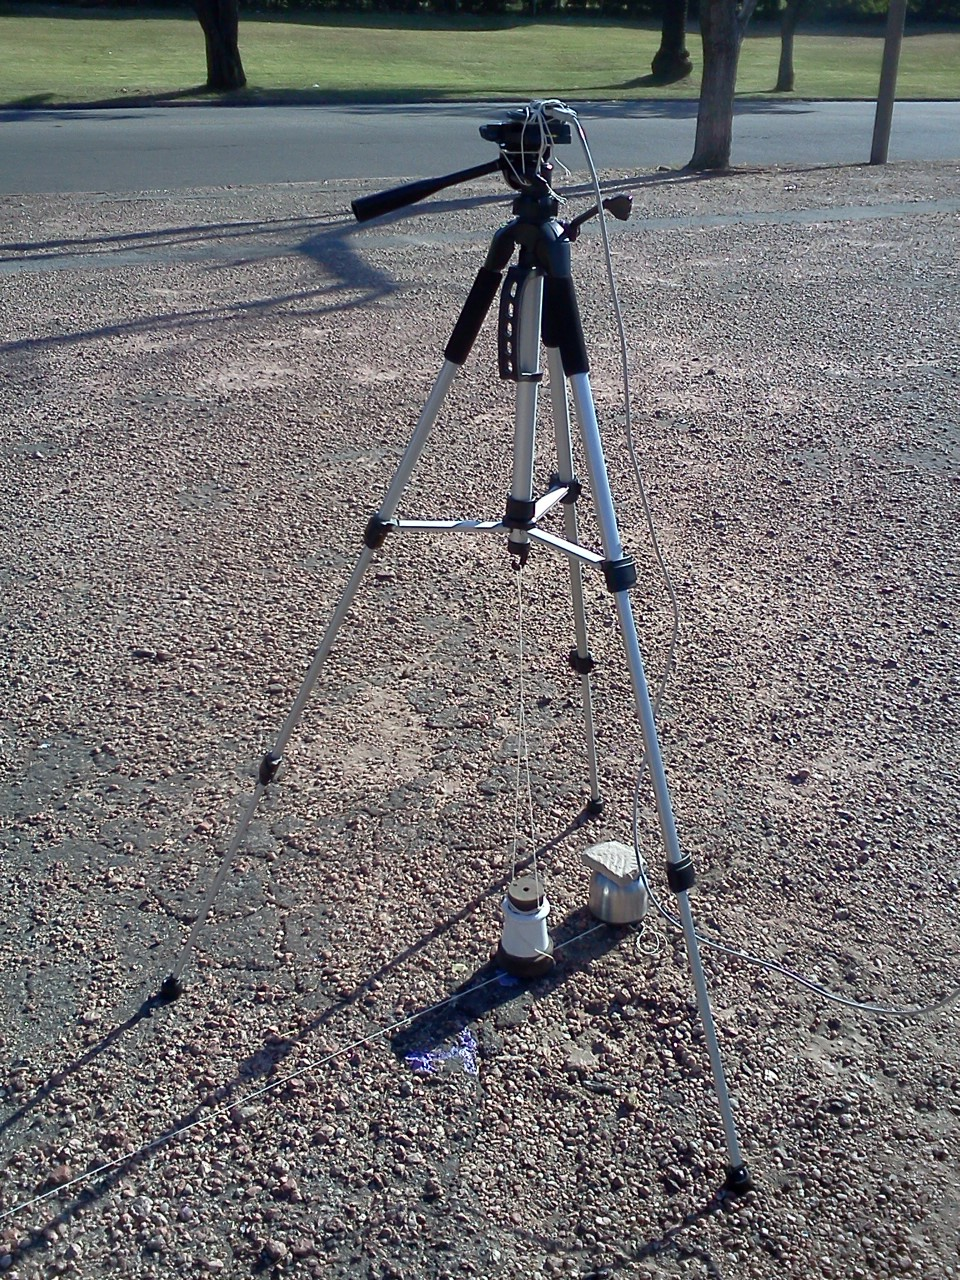
\includegraphics[width=0.2\textwidth]{./pics_gps/tripode_con_plomada.jpg}}
  \subfloat[]{\label{fig:vista_usb.jpg}
    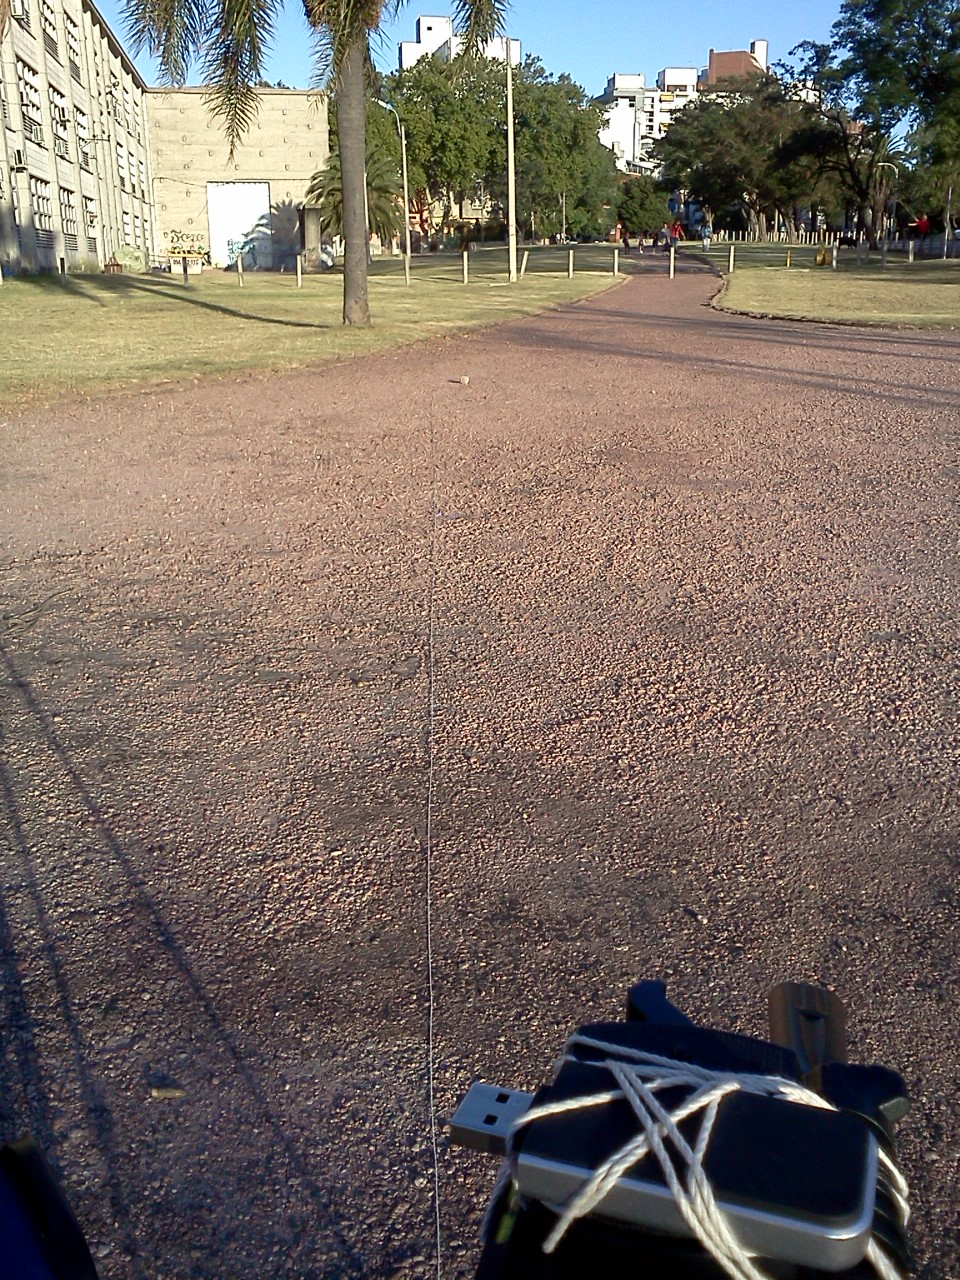
\includegraphics[width=0.2\textwidth]{./pics_gps/vista_usb.jpg}}
\vspace{-10pt}
  \caption{GPS y Atril}
  \label{fig:rebotes}
  \vspace{-20pt}
\end{wrapfigure}

En la figura \ref{fig:tripode_con_plomada.jpg} se observa el trípode que sostiene al GPS. Se busca tener el GPS a una altura fija, y separado del piso. Al nivel del piso los rebotes degradan seriamente la performance del GPS. La cuerda que marca el lado del polígono, junto con las patas del trípode, se utilizaron para fijar la orientación del GPS durante el experimento.

\subsection{Adquisición de datos}
\label{sec:adquisicion-de-datos}

Para tomar datos se conectó el GPS, que env\'ia información mediante USB-serie, al puerto USB de una computadora. En la computadora se utilizó \textit{GPSD}\footnote{\url{http://catb.org/gpsd/}}, un software open-source que hace de \textit{daemon}, y se encarga de transformar los datos del GPS a una estructura fácil de manejar en \verb+C+.

El GPS emite sentencias NMEA a través de un puerto USB serie, a 38400bps. Trabaja con sentencias:
\begin{itemize}
\item GPGGA - \textit{Global Positioning System Fix Data}: Información sobre la fecha, posición y datos relevantes sobre el \textit{fix}.
\item GPGSV - \textit{Satellites in view}: Información sobre la cantidad de satélites detectados, y la calidad de la se\~nal proveniente de cada uno.
\item GPGSA - \textit{DOP and active satellites}: Información sobre DOP\footnote{\textit{Dilution of precision} - Ver \ref{sec:dop}.} y satélites activos.
\item GPRMC - \textit{Recommended minimum specific GPS/Transit data}: Sentencia mínima recomendada, trae suficiente información como para poder trabajar con el GPS.
\item GPVTG - \textit{Track Made Good and Ground Speed}: Información sobre la dirección y la velocidad (\textbf{no} sobre la posición absoluta).
\end{itemize}

\subsection{Verificación del polígono}
\label{sec:verificacion-del-poligono}

\begin{wraptable}{r}{0.5\textwidth}
\centering
\vspace{-25pt}
\caption{Diagonales del polígono (cm).}\label{tab:diagonales-poligono}
\begin{tabular}{|c|c|c|c|c|}
\hline
\rowcolor[gray]{0.9}
\textbf{D12} & \textbf{D13} & \textbf{D14} & \textbf{D15} & \textbf{D16} \\
\hline
603 & 1205 & 606 & 855 & 1345 \\
\hline
\rowcolor[gray]{0.9}
\textbf{D23} & \textbf{D24} & \textbf{D25} & \textbf{D26} & \textbf{D34} \\
\hline
603 & 853 & 608 & 853 & 1344\\
\hline
\rowcolor[gray]{0.9}
\textbf{D35} & \textbf{D36} & \textbf{D45} & \textbf{D46} & \textbf{D56} \\
\hline
850 & 602 & 602 & 1202 & 603 \\
\hline
\end{tabular}
\vspace{-30pt}
\end{wraptable}

Una vez construido el polígono, es de interés medir todas las diagonales (con la cinta métrica) por dos motivos:
\begin{itemize}
\item Verificar que no se cometieron errores.
\item Hacer mínimos cuadrados con las medidas, de manera de obtener un polígono, que no tiene porqué ser (y en general no será) un rectángulo, sino algo similar a un rectángulo, más ajustado a la realidad.
\end{itemize}

\begin{wrapfigure}{r}{0.6\textwidth}
\vspace{-20pt}
  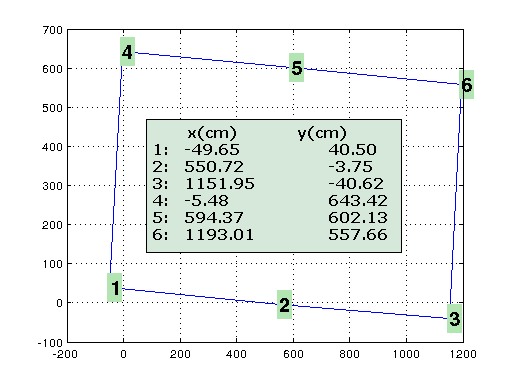
\includegraphics[width=.5\textwidth]{./pics_gps/pol_mc.png}
\caption{Polígono luego de MC.}
\label{fig:pol_mc.png}
\vspace{-20pt}
\end{wrapfigure}
Las medidas tomadas se resumen en la tabla \ref{tab:diagonales-poligono}, donde \verb+D12+ representa la medida de la recta que une el punto \verb+1+ con el punto \verb+2+, en cm.

El polígono resultante se observa en la figura \ref{fig:pol_mc.png}. El error relativo, es decir, el cociente entre las medidas de cada recta \textbf{DAB} (distancia entre el punto \verb+A+ y el \verb+B+) resultante de aplicar MC, y lo esperado en el polígono teórico, de 6m de lado, es:

\begin{itemize}
\item $9.51\%$ en el peor caso.
\item $4.65\%$ en promedio.
\end{itemize}

Se puede trabajar con el pol\'igono irregular que fue efectivamente construido en el resto del experimento, pero la interpretación de los resultados se torna poco intuitiva. Considerando que el error es inferior al 10\% en el peor caso, se opta por continuar el experimento considerando que el pol\'igono es un rect\'angulo de lados 12 y 6 metros.

\subsection{Punto fijo - 2 minutos}
\label{sec:gps2-punto-fijo-2-minutos}

Se tomaron datos durante aproximadamente 2 minutos ($\approx$ 120 muestras) en cada uno de los vértices del polígono, con el objetivo de observar la estabilidad de la información proveniente del GPS.

\begin{wrapfigure} {r} {0.6\textwidth}
\vspace{-10pt}
  \centering
  \subfloat[Orientación \#3]{\label{fig:or2.jpg}
    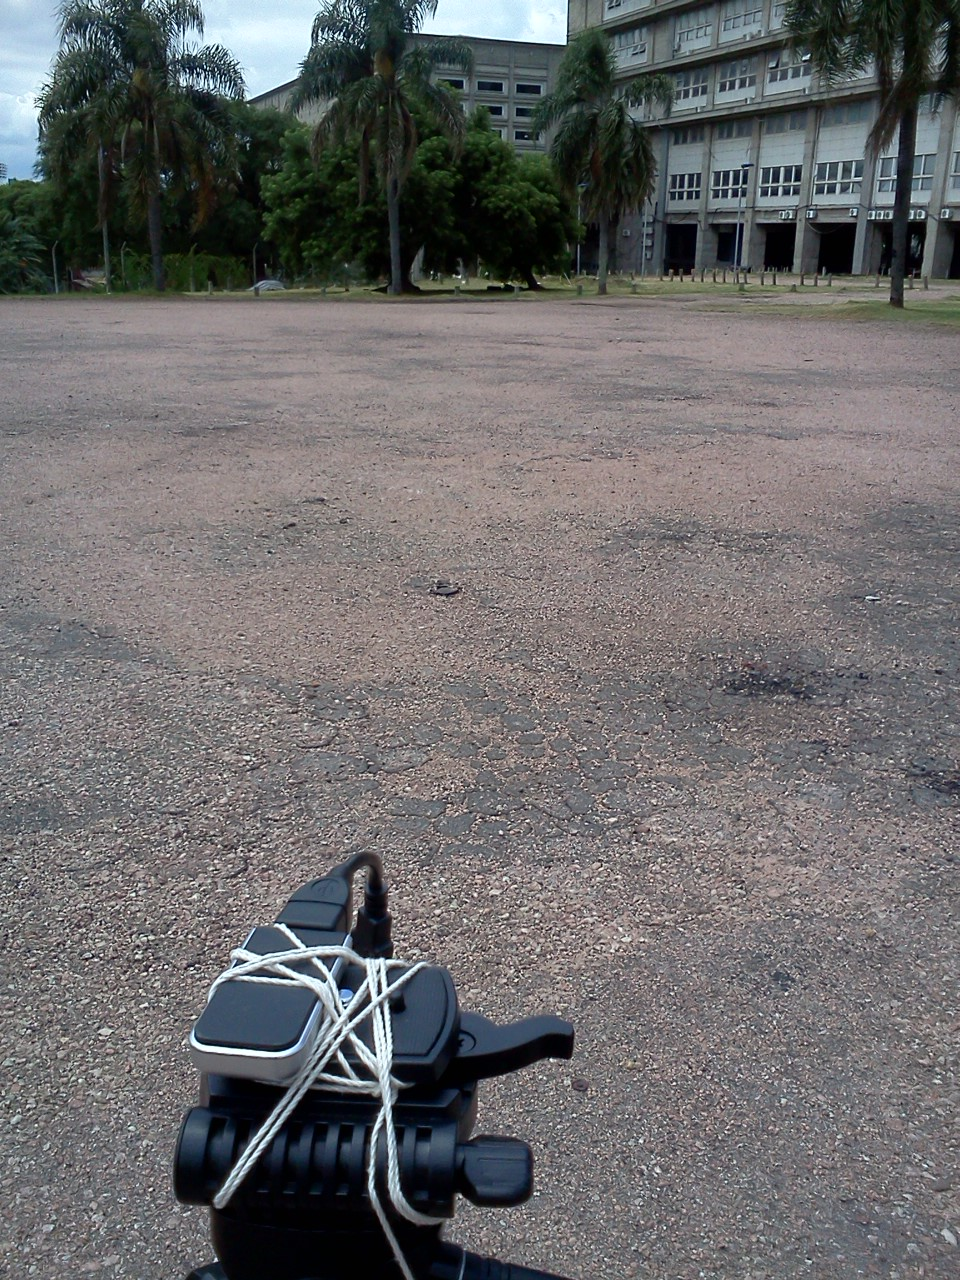
\includegraphics[width=0.27\textwidth]{./pics_gps/or2.jpg}}
  \subfloat[Orientación \#1 y \#4.]{\label{fig:or3.jpg}
    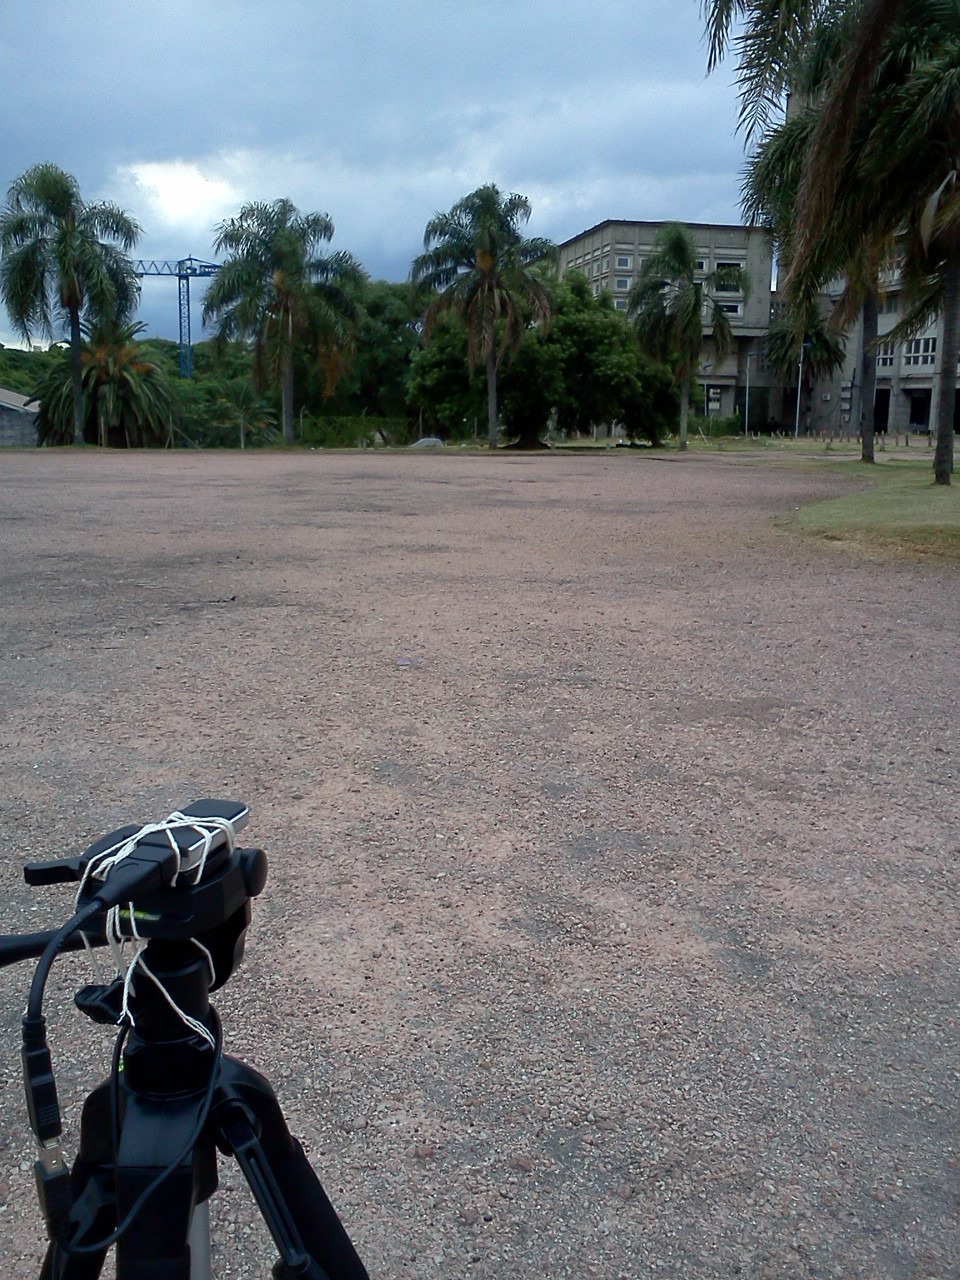
\includegraphics[width=0.27\textwidth]{./pics_gps/or3.jpg}}
\vspace{-10pt}
\caption{Orientaciones del GPS}
\vspace{-20pt}
\end{wrapfigure}

En las figuras \ref{fig:or2_todos_sat_mal.png} y \ref{fig:punto_fijo_dos_minutos} se muestra el error en los datos del GPS respecto al valor promedio. Si este careciera de error relativo, todas las muestras coincidirían con el promedio, y estarían ubicadas en el punto \verb+[0,0]+. En dichas figuras la circunferencia negra es de 2.5m de radio. En la leyenda se muestra qué porcentaje de las muestras se encuentran fuera del círculo. Se Repite el experimento tomando datos durante 10 minutos por punto obteniendo resultados similares. Se orientó el GPS de 3 maneras distintas, siempre alineando el trípode con uno de los lados de 12m del rectángulo:

\begin{enumerate}
\item USB hacia la calle, LED hacia el estacionamiento, como en la figura \ref{fig:or3.jpg}.
\item USB hacia la rambla, LED hacia el IIE (no hay figura)
\item Como en la figura \ref{fig:or2.jpg}.
\item Nuevamente, USB hacia la calle, LED hacia el estacionamiento, como en la figura \ref{fig:or3.jpg}.
\end{enumerate}

\begin{figure}[h!]
\caption{Punto fijo - 2 minutos}
  \hspace{-50pt}
  \subfloat[Orientación: \textbf{4}.]{\label{fig:2m_or1_todos.png}
    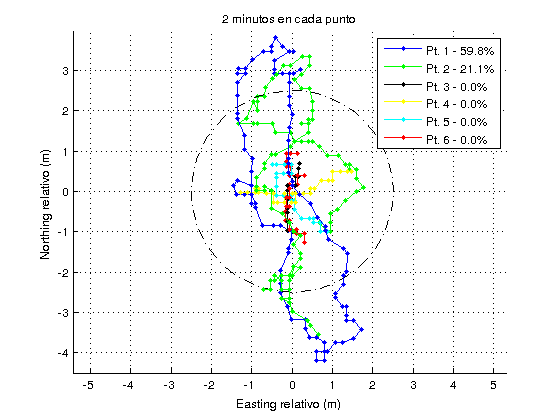
\includegraphics[width=.6\textwidth]{./pics_gps/2m_or1_todos.png}}
  \subfloat[Orientación: \textbf{2}.]{\label{fig:2m_or2_todos.png}
    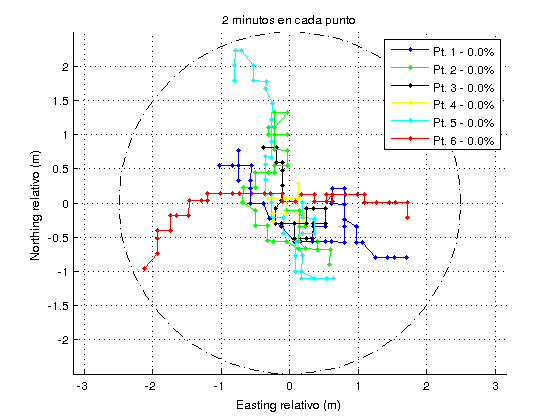
\includegraphics[width=.6\textwidth]{./pics_gps/2m_or2_todos.png}}\\

  \hspace{-50pt}
  \subfloat[Orientación: \textbf{3}.]{\label{fig:or2_todos_cut.png}
    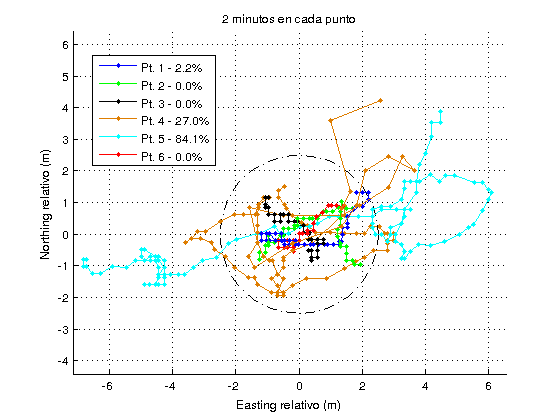
\includegraphics[width=.6\textwidth]{./pics_gps/or2_todos_cut.png}}
  \subfloat[Orientación: \textbf{4}]{\label{fig:or3_todos.png}
    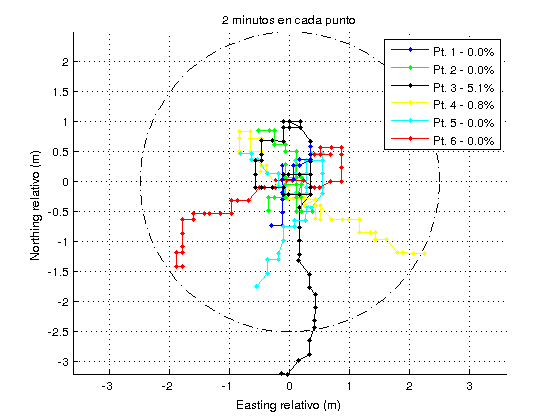
\includegraphics[width=.6\textwidth]{./pics_gps/or3_todos.png}}
\vspace{-20pt}
\label{fig:punto_fijo_dos_minutos}
\end{figure}

\vspace{-20pt}
\subsubsection{Punto fijo: Análisis - \textbf{satélites disponibles}}
\label{sec:gps2-punto-fijo-analisis-sat-count}

\begin{wrapfigure}{r}{0.65\textwidth}
\vspace{-25pt}

  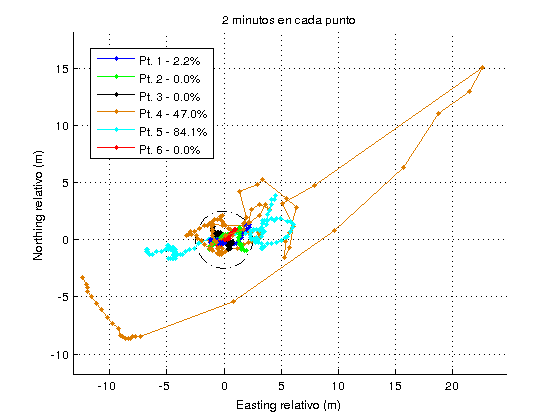
\includegraphics[width=.55\textwidth]{./pics_gps/or2_todos_sat_mal.png}
  \vspace{-15pt}
  \caption{Datos con solamente 4 satélites. Orientación: \textbf{3}.}
  \label{fig:or2_todos_sat_mal.png}
\end{wrapfigure}
La teoría dice que con 4 satélites debería alcanzar para obtener un \textit{fix 3D}, es decir, estimar la posición sobre la esfera terrestre, y la distancia (altura) a la misma. Se recomienda tener no menos de 6 sat\'elites. Durante el experimento de la figura \ref{fig:or2_todos_cut.png}, hubo un per\'iodo de tiempo en el cual el GPS perdió la se\~nal, y el número de satélites disponibles, que usualmente es 9 o 10, pasó a ser 4. Los datos correspondientes se muestran en la figura \ref{fig:or2_todos_sat_mal.png}. El trazo naranja, con un error de hasta 23 metros, corresponde a instantes donde la cantidad de satélites era entre 4 y 5. Luego de volver a 9 o 10 satélites, los datos tienen errores razonables.\\



En la figura \ref{fig:or2_todos_cut.png} se observa el mismo log que en \ref{fig:or2_todos_sat_mal.png}, pero luego de haber quitado las muestras correspondientes al período donde se deterioró la se\~nal. No se pudo encontrar una explicación para la mala calidad de las muestras correspondientes al punto 5 en la figura \ref{fig:or2_todos_cut.png}. La cantidad de satélites disponibles se mantuvo estable en 9 o 10 durante la adquisición de los datos.

\subsubsection{Punto fijo: Análisis - \textbf{Orientación}}
\label{sec:gps-orientacion}

Para evaluar si existe una correlación entre la orientación y las medidas del GPS, se hizo el siguiente experimento:
\begin{enumerate}
\item Tomar datos durante 10 minutos con el GPS arriba del trípode, dos patas alineadas con una recta fija.
\item Rotar el trípode 120 grados en sentido horario, de manera que otro lado del triángulo que forman las patas del trípode quede alineado con la recta. Tomar datos durante 10 minutos.
\item Rotar y tomar datos nuevamente.
\end{enumerate}

Los resultados del experimento se observan en la figura.

\begin{figure}[h!]
\hspace{-70pt}
  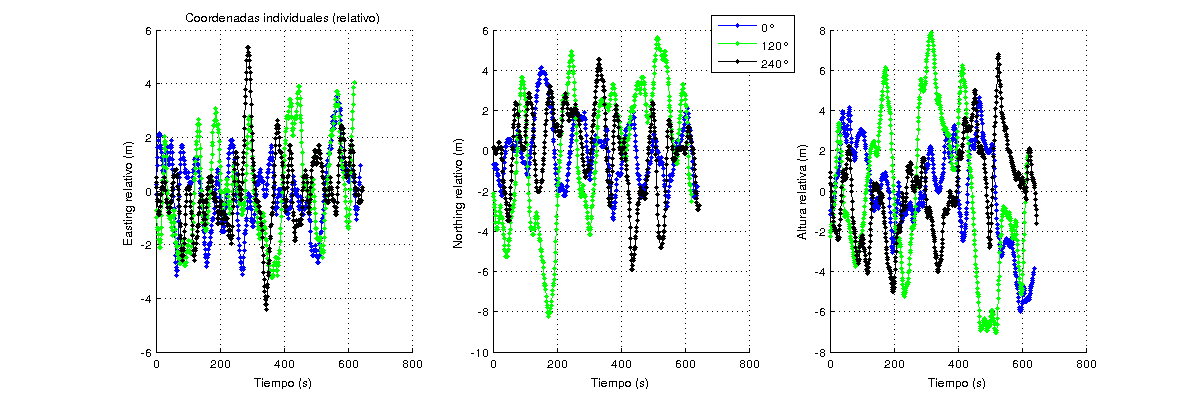
\includegraphics[width=1.4\textwidth]{./pics_gps/orientacion_individual.png}
  \caption{Datos rotando el GPS sobre un punto fijo.}
  \label{fig:orientacion_individual.png}
\end{figure}

\subsubsection{Orientación - Conclusiones}
\label{sec:orientacion-conclusiones}

No se encontró una correlación entre la orientación del GPS y el error en las medidas.
El experimento se realizó con cielo abierto, con una buena geometría, en términos de distribución de satélites. Tal vez en situaciones de visibilidad limitada se podría observar una correlación, ya que si la dirección en la que la antena recibe mejor coincide con el lugar donde hay pocos satélites, entonces la cantidad de información sería menor/peor que en otras orientaciones.

Tener visibilidad limitada por obstáculos, o tener una mala geometría deteriora la performance del GPS. En este trabajo no se considerar\'a la situaci\'on en la cual se tiene una performance deficiente, o bien se utilizar\'a el GPS a cielo abierto, o se trabajar\'a bajo techo (sin GPS).

%El impacto de la geometría se analiza en la sección \ref{sec:geometria}.

\subsection{Polígono}
\label{sec:gps2-poligono}

En la figura \ref{fig:10min_pol.png}, la línea en roja representa el polígono resultante de unir el promedio en cada vértice de las muestras tomadas durante un experimento de 10 minutos. En la figura \ref{fig:10m_mapa.png} se dicho polígono, proyectado sobre una foto satelital\footnote{El mapa y las fotos se obtuvieron de:\\ \url{http://sig.montevideo.gub.uy/mapas/mapa-principal}}.

\begin{figure}[h!]
\vspace{-10pt}
  \centering
  \subfloat[Polígono formado por los promedios de 10 minutos.]{\label{fig:10min_pol.png}
    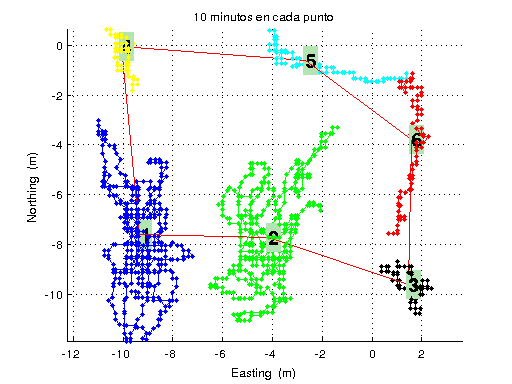
\includegraphics[width=.4\textwidth]{./pics_gps/10min_pol.png}}
  \subfloat[Proyección del polígono sobre una foto satelital.]{\label{fig:10m_mapa.png}
    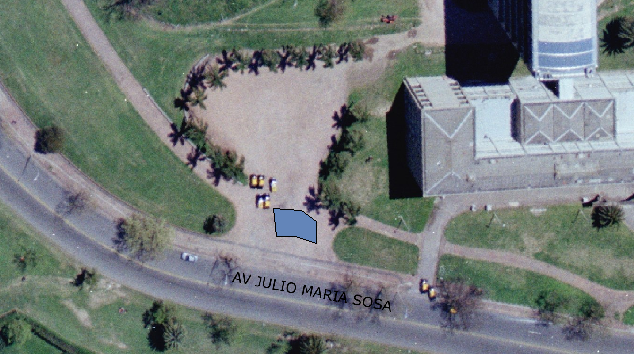
\includegraphics[width=.4\textwidth,height=.28\textwidth]{./pics_gps/10m_mapa.png}}
\vspace{-10pt}
\caption{Polígono}
\vspace{-10pt}
\end{figure}

En las siguientes figuras se observan los polígonos formados por los promedios de varias secuencias de 2 minutos por punto. 

\begin{figure}[h!]
\vspace{-10pt}
  \centering
\subfloat[Orientación: \textbf{4}.]{\label{fig:2m_or1_pol.png}
  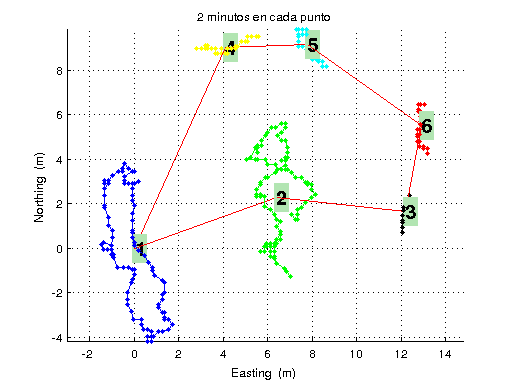
\includegraphics[width=.5\textwidth]{./pics_gps/2m_or1_pol.png}}
\subfloat[Orientación: \textbf{2}.]{\label{fig:2m_or2_pol.png}
  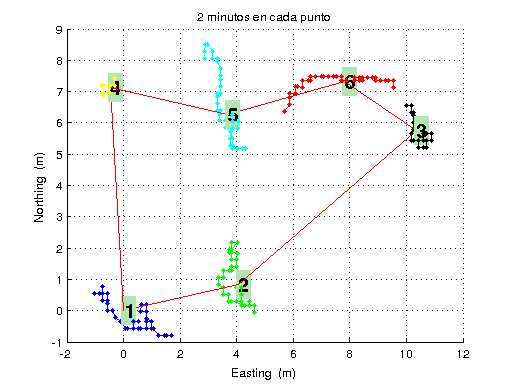
\includegraphics[width=.5\textwidth]{./pics_gps/2m_or2_pol.png}}\\  
\subfloat[Orientación: \textbf{3}.]{\label{fig:or2_poly_cut.png}
  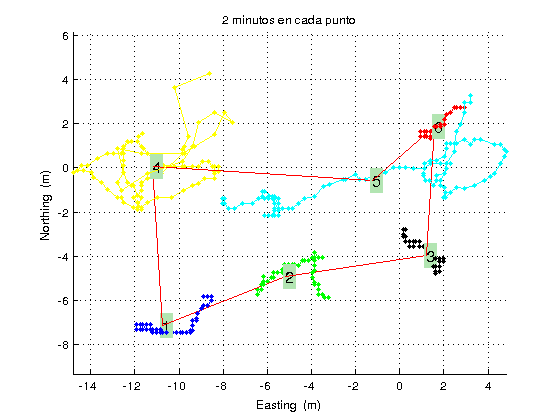
\includegraphics[width=.5\textwidth]{./pics_gps/or2_poly_cut.png}}
\subfloat[Orientación: \textbf{4}]{\label{fig:or3_pol.png}
  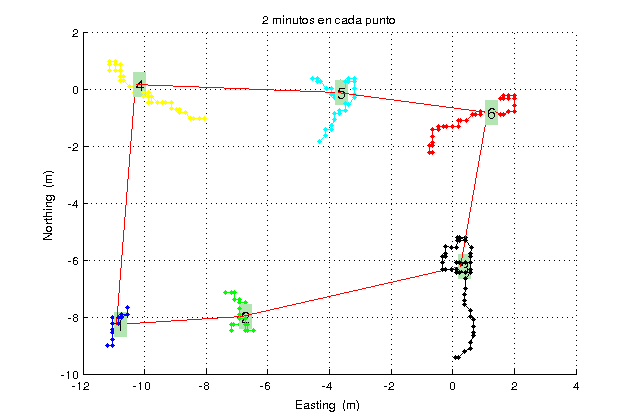
\includegraphics[width=.5\textwidth]{./pics_gps/or3_pol.png}}
\vspace{-10pt}
\caption{Polígono - 2 minutos por punto}
\vspace{-10pt}
\end{figure}

\subsection{Polígono - Análisis}
\label{sec:poligono-analisis}

Dado que no se cuenta con una referencia absoluta, como podría serlo un GPS de alto nivel, no es posible hablar de error absoluto. De cualquier forma, con la información disponible es posible obtener un estimador del error típico en una distancia de \verb+X+ metros, donde \verb+X+ pertenece al conjunto de las medidas de las rectas en juego: \verb+{6;8.5;12;13.45}+ metros. Se comparan las distancias entre los vértices del polígono experimental, con las distancias entre las coordenadas resultantes de la aplicación de mínimos cuadrados a las medidas efectuadas con el metro (ver la sección \ref{sec:verificacion-del-poligono}).

El error relativo para cada recta resulta:

\begin{equation}
  \label{eq:gps-err-rel}
  E = \left|\|\hat{P}_{i} - \hat{P}_{j}\| - D_{ij}\right|
%  E = \frac{1}{N}\sum_{i=1}^{5}\sum_{j=i+1}^6\left|\|\hat{P}_{i} - \hat{P}_{j}\| - D_{ij}\right|
\vspace{-5pt}
\end{equation}
Donde:
\begin{itemize}
\item $\hat{P}_i$ es la dupla \verb+{x,y}+, coordenadas experimentales del i-ésimo vértice del polígono.
\item $D_{ij}$ es la distancia entre el i-ésimo y el j-ésimo vértice, resultado de la aplicación de MC en la sección \ref{sec:verificacion-del-poligono}.
\end{itemize}

Para cada set de estimaciones de la posición de los vértices del polígono\footnote{Un set de valores $\hat{P}_1^1,\hat{P}_2^1,\hat{P}_3^1,\hat{P}_4^1,\hat{P}_5^1,\hat{P}_6^1$}, se utilizó la fórmula \ref{eq:gps-err-rel}, separando los datos según el largo esperado de la recta\footnote{Valores posibles: \{6;8.5;12;13.45\}}. Resulta un set de valores del ``\textit{error al estimar la distancia entre dos puntos que deberían estar a X metros}'', para cada valor de \verb+X+. 

Los resultados se resumen en la tabla \ref{tab:err-rectas}.

\begin{table}[H]
\vspace{-10pt}
\begin{center}
\begin{tabular}{|c|c|c|c|c|}
\hline
\textbf{Largo Teo. (cm)} & $\mu$ (cm) & $\sigma$ (cm)  & $\frac{\mu + 2\sigma}{\text{Largo Teo.}}$ & \textbf{\# Muestras} \\
\hline
\rowcolor[gray]{0.9}
600 & 372.15 & 169.39 & 118\% & 35\\
\hline
\rowcolor[gray]{0.8}
848 & 493.6 & 165.79 & 97\%& 20\\
\hline
\rowcolor[gray]{0.9}
1200 & 429.67 & 212.81 & 71\% & 10\\
\hline
\rowcolor[gray]{0.8}
1341 & 614.73 & 166.71 & 70\% & 10\\
\hline
\end{tabular}
\caption{}
\label{tab:err-rectas}
\end{center}
\vspace{-30pt}
\end{table}

En la tabla \ref{tab:err-rectas} se observa, cómo es de esperarse, que el error relativo disminuye al intentar estimar distancias mayores. Asumiendo que el error en la estimación de la posición de cada punto \verb+A+, \verb+B+ es similar, entonces para cometer un error de \verb+P+\% en la estimación de una distancia \verb+X+ (medida con el metro) entre \verb+A+ y \verb+B+, el GPS debe equivocarse en $\frac{P}{100}X\frac{1}{2}$ en la estimación de la posición de \verb+A+ y \verb+B+.

Resulta que el error en la estimación de la distancia entre dos puntos es aproximadamente 4.5m. Esto es coherente con los resultados sobre la estimación de un punto fijo. Si las medidas para la posición de un punto fijo en general caen dentro de un círculo de 2.5m de radio, entonces, el error en el peor caso en la distancia es de 5m.

Nuevamente, no se cuenta con información sobre la posición real, pero parece razonable asumir que la ubicación real es cercana al promedio de los datos provenientes del GPS. Evidencia a favor de esto se observa en la figura \ref{fig:10m_mapa.png}. En la sección \ref{sec:posicion-absoluta} se profundiza en este aspecto.

\vspace{-20pt}
\section{Caminata por el borde del polígono}
\label{sec:caminata-por-el-borde-del-poligono}

Para simular una situación más parecida a la que se tendrá con el GPS montado sobre el cuadricóptero, se colocó el trípode con el GPS en un mochila, y se procedió a recorrer el polígono con con la mochila puesta.

Los errores en la medida de un punto fijo hacen pensar que sería posible que la trayectoria determinada por el GPS luego de este experimento fuese similar a un rectángulo.

En las figuras siguientes se observan los datos tomados durante 3 caminatas siguiendo el contorno del polígono, siguiendo la secuencia \verb+1-2-3-6-5-4-1+\footnote{Notar que \textbf{no} se recorre en el mismo orden en el que se numeran los puntos del rectángulo}. Se empezó a loguear datos en el punto 1, y se terminó nuevamente en el punto 1.

\begin{figure} [h!]
\vspace{-10pt}
  \centering
  \subfloat[Caminata \#1]{\label{fig:caminata1.png}
    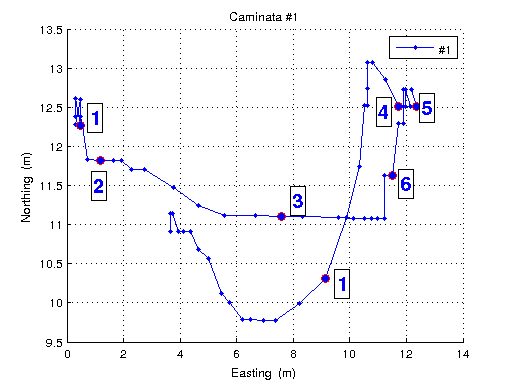
\includegraphics[width=0.4\textwidth]{./pics_gps/caminata1.png}}
  \subfloat[Caminata \#2]{\label{fig:caminata2.png}
    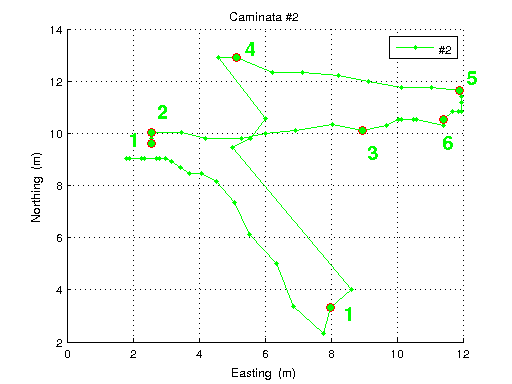
\includegraphics[width=0.4\textwidth]{./pics_gps/caminata2.png}}
  \label{fig:caminatas}
\caption{Caminatas por el borde del polígono}
\vspace{-20pt}
\end{figure}

\newpage
\subsection{Caminata - Análisis}
\label{sec:caminata-analisis}

\begin{wrapfigure}{r}{0.5\textwidth}
  \begin{center}
\vspace{-30pt}
    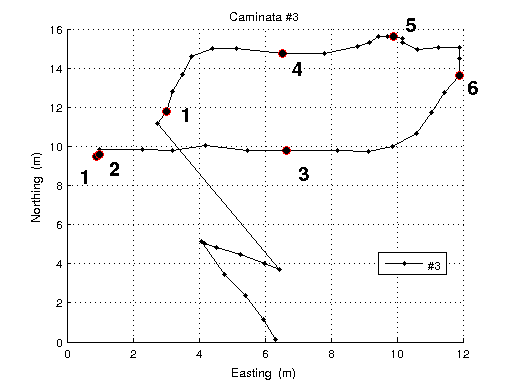
\includegraphics[width=0.5\textwidth]{./pics_gps/caminata3.png}
  \end{center}
\vspace{-20pt}
  \caption{Caminata \#3}
  \label{fig:caminata3}
\vspace{-10pt}
\end{wrapfigure}

Las gráficas de las caminatas son muy desalentadoras. Se observa un error mayor al esperado a partir de los experimentos de punto fijo. Recorrer el pol\'igono no es comparable a tomar muestras, quieto, en cada v\'ertice.

En algunos de los experimentos la posición parece tender a estabilizarse una vez que se llega al destino final, el punto 1. Ahí se continuó logueando datos por unos 20 segundos. En la figura \ref{fig:caminata2.png} la posición final parece tener un drift que se aleja de la posición inicial, en lugar de acercarse. No se encontró una justificación para este comportamiento.

\section{Error en altura}
\label{sec:error-en-altura}

Para determinar el error la información sobre la altura que provee el GPS, se dise\~nó un experimento, que consiste en tomar medidas en una perpendicular a la esfera terrestre, a 4 alturas diferentes: 0m, 1m, 2m y 3m respecto al suelo.

\begin{wrapfigure}{r}{0.6\textwidth}
\vspace{-30pt}
  \begin{center}
  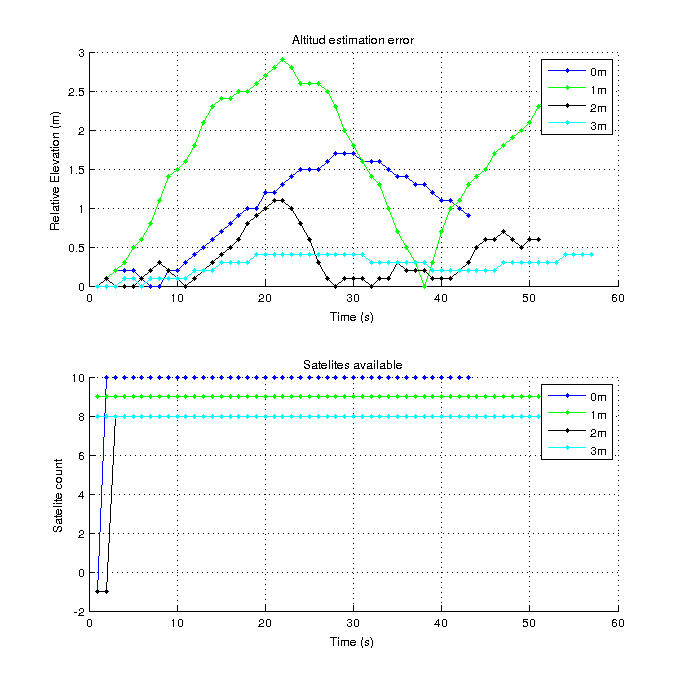
\includegraphics[width=.5\textwidth]{./pics_gps/altura_punto_fijo_fing.png}
  \end{center}
\vspace{-25pt}
  \caption{Variación de la altura determinada por el GPS a distintas alturas.}
  \label{fig:altura_punto_fijo_fing.png}
\vspace{-15pt}
\end{wrapfigure}

Se mantuvo el GPS quieto en cada uno de los niveles, y se tomaron muestras durante aproximadamente 60 segundos. El objetivo de esta etapa era verificar si era viable el experimento.

Se colocó una escalera en el medio del estacionamiento de atrás de la Facultad de Ingeniería, se ató un piolín con marcas cada 1 metro, y una plomada en la punta para mantenerlo tenso y vertical.

En la figura \ref{fig:altura_punto_fijo_fing.png} se observan los resultados del experimento. Es de esperarse que el error sea mayor al estar apoyado sobre el suelo, ya que los rebotes (\textit{multipath}) pueden deteriorar el sistema. El error a 1m de altura es mayor al que se obtuvo con el GPS en el suelo, una posible explicación para esto sería que el GPS estaba muy cerca de la escalera metálica, lo cual podría introducir una cantidad significativa de rebotes.

Los resultados de este experimento llevan a pensar que el GPS da información estable si se encuentra a al menos 2m del suelo. Esto no parece ser un problema, ya que el cuadricóptero volará a alturas superiores.

\section{Tiempo de \textit{warmup}}
\label{sec:tiempo-de-warmup}

El tiempo que demora el GPS en adquirir un \textit{fix} depende de si estaba apagado, o si estaba previamente en funcionamiento.
\begin{itemize}
\item \textbf{Frío}: Aproximadamente 40 segundos.
\item \textbf{Caliente}: Entre 3 y 5 segundos.
\end{itemize}

Esto implicaría que al prender el cuadricóptero, habría que esperar unos 40 segundos para obtener se\~nal del GPS, y que si por algún motivo se pierde la conexión con el GPS, habrá que esperar entre 3 y 5 segundo antes de contar con datos útiles nuevamente.

\section{Tasa de muestreo}
\label{sec:tasa-de-muestreo}

El GPS bajo funcionamiento normal trabaja a aproximadamente 1Hz. Se observ\'o un patr\'on de 3 muestras a 1Hz, luego una 4ta muestra pegada a la \'ultima de las 3, luego nuevamente a 1Hz.

Se observó que estando quieto, a veces repite información, y la etiqueta como ``válida''. Se observó este comportamiento durante los experimentos de punto fijo, llegando a pasar 30 segundos registrando exactamente la misma información.

Se compararon los datos crudos provenientes del GPS con los que devuelve el GPSD, y se concluyó que el GPSD \textbf{no} es responsable de la repetición de datos, es decir, no es un problema de software, sino que el GPS es quien env\'ia datos repetidos.

Al loguear trayectorias de movimiento permanente, como un recorrido en bicicleta de 15 minutos, no se observaron  datos repetidos durante más de 4 segundos. No parece razonable que el cálculo de la posición dé \textit{exactamente} lo mismo durante varias medidas sucesivas, probablemente se trate de un problema interno del GPS.

\section{Posición Absoluta}
\label{sec:posicion-absoluta}

\begin{wrapfigure}{r}{0.5\textwidth}
  \begin{center}
\vspace{-80pt}
  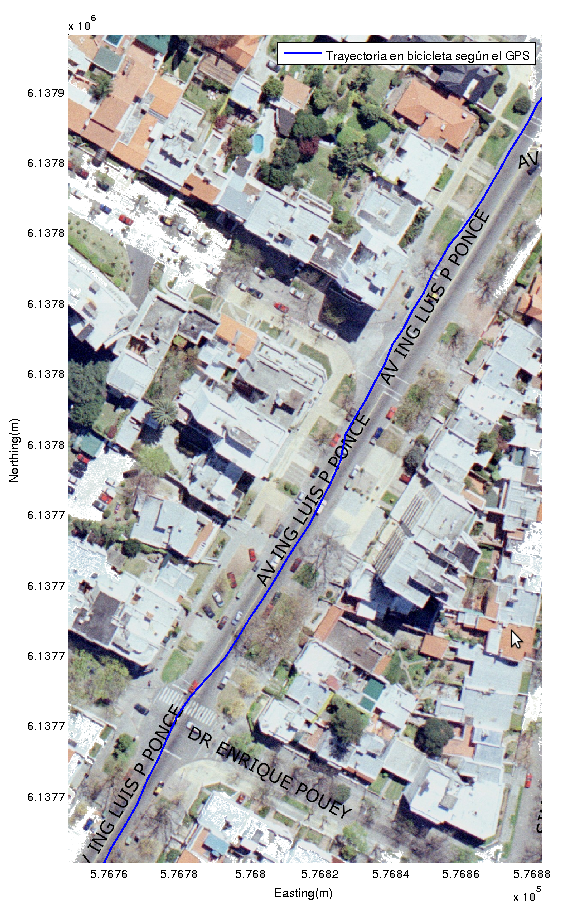
\includegraphics[height=.5\textwidth]{./pics_gps/ponce.png}
  \end{center}
\vspace{-20pt}
  \caption{Recorrido en bicicleta.}
  \label{fig:ponce.png}
\vspace{-10pt}
\end{wrapfigure}

Se realizaron varios experimentos para analizar si la ubicación que daba el GPS se correspondía con la realidad, ya que algunos GPSs a veces dan un error constante de varios metros, y de ser el caso, se podría considerar este offset.

Sobre un mapa de Montevideo se graficaron trayectorias conocidas, con el objetivo de verificar que los datos provenientes del GPS eran ``razonables''.

No se observo un corrimiento de los datos evidente y constante, por lo que se asume el GPS \textbf{no} introduce un offset.

En la figura \ref{fig:ponce.png} se observa una trayectoria realizada en bicicleta, con el GPS colocado sobre el trípode, asomando de una mochila. El recorrido fue hacia el sur-oeste, sobre el cord\'on nor-oeste. Se observa que la posici\'on dada por el GPS marca un camino similar al realizado, pero a veces llega a cruzar al cord\'on opuesto (esto no sucedi\'o durante el experimento).

\section{Conclusiones}
\label{sec:conclusion}

Los siguientes items servirán de guía para la utilización del GPS como instrumento de navegación:

\begin{itemize}
\item \textbf{Error en las medidas}: Las medidas del GPS tienen un error t\'ipico menor a 2.5m para un punto fijo, situaci\'on irreal, ya que el cuadric\'optero necesita al GPS para poder quedarse quieto. Para las caminatas el error es de alrededor de \textbf{5m}, siempre que se disponga de una buena geometr\'ia y de alrededor de 9-10 sat\'elites a la vista. Es de esperarse que la performance se reduzca al utilizar el GPS montado sobre el cuadr\'icoptero, donde estar\'a sujeto a interferencia electromagnética de los motores, vibraciones, etc.
\item \textbf{Visibilidad}: Es importante asegurar buena visibilidad, la performance del GPS se reduce drásticamente si pierde satélites.
\item \textbf{Resolución}: El GPS \textbf{no} es adecuado para tareas de navegación con restricciones menores a 10 metros, pero sí para distancias de varias decenas de metros.
\item \textbf{Tasa de muestreo}: El GPS normalmente muestrea a \textbf{1Hz}. Cabe destacar que debe ignorarse información repetida (muestras sucesivas que sea idénticas).
\item \textbf{Error en altura}: El GPS \textbf{no} es adecuado para determinar la elevación durante el aterrizaje/despegue, ya que a menos de 2m del piso, la estimación de la elevación es muy mala. Será necesario otro sensor (sensor de presión, IR, etc) para asistir durante el despegue/aterrizaje.
\item \textbf{Tiempo de \textit{fix}}: En frío demora alrededor de 40 segundos, en caliente entre 3 y 5 segundos.
\end{itemize}


\end{document}